\documentclass{report}
\usepackage[utf8]{inputenc} %encodage entrée
\usepackage{endnotes} %notes de fin
\usepackage{graphicx} %images
\usepackage[usenames,dvipsnames]{color} %couleurs
\usepackage{listings} %mise en forme de code source
\usepackage{xfrac}
\renewcommand\theequation{\arabic{equation}}
\usepackage{tabularx} % modifier la taille des cellules des tableaux
\usepackage{upquote}
\usepackage{textcomp}
\usepackage{pdfpages}
\usepackage[frenchb]{babel} %langue
\usepackage{amsmath} %affichage des matrices
\usepackage{lipsum} %génération de lipsum
\usepackage{verbatim} %code source
\usepackage{moreverb} %amélioration du package verbatim
\usepackage{titlesec} %formatage des chapitres
\titleformat{\chapter}[hang]{\bf\huge}{\thechapter}{2pc}{}
\usepackage[a4paper]{geometry} %mise en page
% \usepackage{varioref,amssymb,float} % polices 
% \usepackage{pgf,tikz} % permet de créer comme pstricks des figures en code LateX 
% \usetikzlibrary{calc} 
% \usepackage{pgflibraryarrows} % librairie liée à tikz 
% \usepackage{pgflibrarysnakes} 
% \usepackage{xcolor} % module de couleur pour tikz 
\geometry{hscale=0.8,vscale=0.8,centering}
%\lstinputlisting[language=Python, firstline=37, lastline=45]{source_filename.py}
\title{Algorithmes numériques -- Rapport \\ \vspace{0.5cm}Interpolation et Approximation}
\author{Axel Delsol, Pierre-Loup Pissavy}
\date{Décembre 2013}
\lstset{literate=
   {á}{{\'a}}1 {é}{{\'e}}1 {í}{{\'i}}1 {ó}{{\'o}}1 {ú}{{\'u}}1
   {Á}{{\'A}}1 {É}{{\'E}}1 {Í}{{\'I}}1 {Ó}{{\'O}}1 {Ú}{{\'U}}1
   {à}{{\`a}}1 {è}{{\`e}}1 {ì}{{\`i}}1 {ò}{{\`o}}1 {ò}{{\`u}}1
   {À}{{\`A}}1 {È}{{\`E}}1 {Ì}{{\`I}}1 {Ò}{{\`O}}1 {Ò}{{\`U}}1
   {ä}{{\"a}}1 {ë}{{\"e}}1 {ï}{{\"i}}1 {ö}{{\"o}}1 {ü}{{\"u}}1
   {Ä}{{\"A}}1 {Ë}{{\"E}}1 {Ï}{{\"I}}1 {Ö}{{\"O}}1 {Ü}{{\"U}}1
   {â}{{\^a}}1 {ê}{{\^e}}1 {î}{{\^i}}1 {ô}{{\^o}}1 {û}{{\^u}}1
   {Â}{{\^A}}1 {Ê}{{\^E}}1 {Î}{{\^I}}1 {Ô}{{\^O}}1 {Û}{{\^U}}1
   {œ}{{\oe}}1 {Œ}{{\OE}}1 {æ}{{\ae}}1 {Æ}{{\AE}}1 {ß}{{\ss}}1
   {ç}{{\c c}}1 {Ç}{{\c C}}1 {ø}{{\o}}1 {å}{{\r a}}1 {Å}{{\r A}}1
   {€}{{\EUR}}1 {£}{{\pounds}}1
}
\lstdefinestyle{customc}{
   belowcaptionskip=1\baselineskip,
   breaklines=true,
   frame=L,
   xleftmargin=\parindent,
   language=C,
   showstringspaces=false,
   basicstyle=\footnotesize\ttfamily,
   keywordstyle=\bfseries\color{ForestGreen},
   commentstyle=\itshape\color{Plum},
   identifierstyle=\color{NavyBlue},
   stringstyle=\color{Orange},
   numbers=left,
   caption=Code : \lstname,
   captionpos=b,
}
\lstset{
upquote=true,
columns=flexible,
basicstyle=\ttfamily,
}
\addto\captionsfrench{\renewcommand{\figurename}{\textsc{Graphique}}}
\addto\captionsfrench{\renewcommand{\tablename}{\textsc{Tableau}}}
\renewcommand{\thefigure}{\thesection.\arabic{figure}}
\renewcommand{\thetable}{\thesection.\arabic{table}}
\renewcommand{\lstlistingname}{\textsc{Figure}}
\lstdefinestyle{apercu}{
  xleftmargin=2cm,
  xrightmargin=2cm,
  frame=single,
  breaklines=true,
  breakatwhitespace=true,
  breakindent=5pt,
  postbreak=\space,
  captionpos=b,
  escapeinside={\%*}{*)},
  showstringspaces=false,
  caption=Apercu : \lstname,
}
\begin{document}
  \maketitle
  \tableofcontents

  \chapter{Préambule}
    \section{Structure du programme}
    Nous avons conçu un programme principal avec menus, présenté sous la forme suivante :
    \begin{lstlisting}[style=apercu, name=Menu Principal]
Menu principal : Interpolation et Approximation

Entrez n le nombre de points : 2
%*\textit{(Saisie de la série de points...)}*)

%*\textit{(Affichage du tableau correspondant...)}*)
Quelle résolution utiliser ?
1- Newton
2- Neuville
3- Régression Linéaire
4- Approximation par une fonction exponentielle
5- Approximation par une fonction "puissance"
9- Nouvelle série de points (Menu principal)
0- Quitter
Votre choix :
    \end{lstlisting}
  \chapter{Interpolation}
    \section{Méthode de Newton}
      \subsection{Présentation}
	
      \subsection{Programme}
	\lstinputlisting[style=customc]{newton.c}
    \newpage
    \section{Méthode de Neuville}
      \subsection{Présentation}
	
      \subsection{Programme}
	\lstinputlisting[style=customc]{neuville.c}
    \newpage
    \section{Résultats de tests}
      \subsection{Exemple tiré d'un TD}
	\begin{table}[h]
	  \centering
	  \begin{tabular}{| c | c | c | c | c |}
	  \hline 
	  $x_{i}$ & $1$ & $2$ & $3$ & $4$ \\ 
	  \hline 
	  $y_{i}$ & $0$ & $0$ & $0$ & $6$ \\ 
	  \hline 
	  \end{tabular}
	  \caption{Série 1}
	  \label{inter_td3_ex3}
	\end{table}

	Méthode de Newton: $P(x)= -6.00 + 11.00 \cdot x- 6.00 \cdot x^{2}  + 1.00 \cdot x^{3} $

	Méthode de Neuville: $P(x)= -6.00 + 11.00 \cdot x- 6.00 \cdot x^{2}  + 1.00 \cdot x^{3} $
	
	\begin{figure}[h]
	  \centering
	  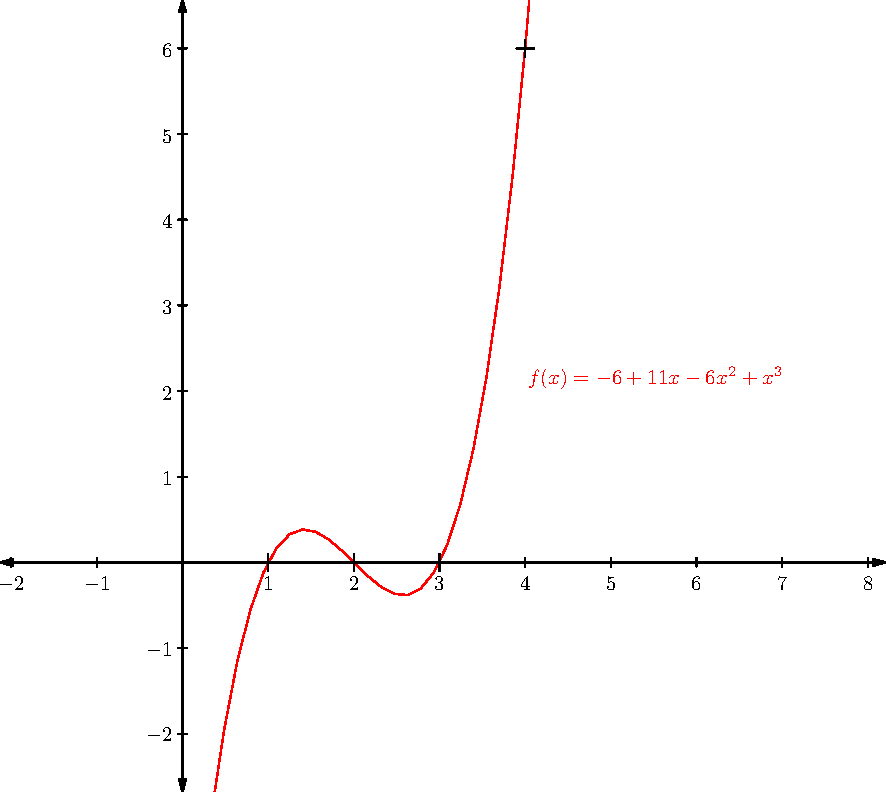
\includegraphics[scale=0.7]{graphiques/pdf_output/inter_test1.pdf}
	  \caption{Interpolation de Newton et Neuville -- (Tableau \ref{inter_td3_ex3})}
	\end{figure}
      \newpage
      
      \subsection{Densité de l'eau en fonction de la température}      
	\begin{table}[h]
	  \centering
	  \begin{tabular}{| c | c | c | c | c | c | c | c | c | c | c |}
	    \hline 
	    $x_{i}$ & $0$ & $2$ & $4$ & $6$ & $8$ & $10$ & $12$ & $14$ & $16$ & $18$ \\
	    \hline 
	    $y_{i}$ & $0.999870$ & $0.999970$ & $1.000000$ & $0.999970$ & $0.999880$ & $0.999730$ & $0.999530$ & $0.999530$ & $0.998970$ & $0.998460$ \\ 
	    \hline 
	  \end{tabular}
	  \begin{tabular}{| c | c | c | c | c | c | c | c | c | c | c |}
	    \hline
	    $x_{i}$ & $20$ & $22$ & $24$ & $26$ & $28$ & $30$ & $32$ & $34$ & $36$ & $38$ \\ 
	    \hline
	    $y_{i}$ & $0.998050$ & $0.999751$ & $0.997050$ & $0.996500$ & $0.996640$ & $0.995330$ & $0.994720$ & $0.994720$ & $0.993330$ & $0.993260$ \\
	    \hline
	  \end{tabular}
	  \caption{Mesures}
	  \label{inter_tp2_ex1_densite}
	\end{table}
	  
	  Méthode de Newton : $P(x)= 0.999870 + 7.693711 \cdot x- 13.276666 \cdot x^{2}  + 9.932303 \cdot x^{3} - 4.345460 \cdot x^{4}  + 1.259124 \cdot x^{5} - 0.258585 \cdot x^{6}  + 0.039240 \cdot x^{7} - 0.004520 \cdot x^{8}  + 0.000402 \cdot x^{9} - 0.000028 \cdot x^{10}  + 0.000002 \cdot x^{11} - 0 \cdot x^{12}  + 0 \cdot x^{13} - 0 \cdot x^{14}  + 0 \cdot x^{15} - 0 \cdot x^{16}  + 0 \cdot x^{17} - 0 \cdot x^{18}  + 0 \cdot x^{19} $
	  
	  Erreur moyenne : $0.000005$

	  Méthode de Neuville : $P(x)= 0.999870 + 7.693711 \cdot x- 13.276666 \cdot x^{2}  + 9.932303 \cdot x^{3} - 4.345460 \cdot x^{4}  + 1.259124 \cdot x^{5} - 0.258585 \cdot x^{6}  + 0.039240 \cdot x^{7} - 0.004520 \cdot x^{8}  + 0.000402 \cdot x^{9} - 0.000028 \cdot x^{10}  + 0.000002 \cdot x^{11} - 0 \cdot x^{12}  + 0 \cdot x^{13} - 0 \cdot x^{14}  + 0 \cdot x^{15} - 0 \cdot x^{16}  + 0 \cdot x^{17} - 0 \cdot x^{18}  + 0 \cdot x^{19} $
	  
	  Erreur moyenne : $0.000033$
		  
	  \begin{figure}[h]
	  \centering
  % 	\includegraphics[scale=0.7]{graphiques/pdf_output/}
	  \caption{Interpolation de Newton et Neuville -- (Tableau \ref{inter_tp2_ex1_densite})}
	\end{figure}
      \newpage
    
      \subsection{3 séries}
	\begin{table}[h]
	  \centering
	  \begin{tabular}{| c | c | c | c | c | c | c | c | c | c | c | c |}
	    \hline 
	    $x_{i}$ & $10$ & $8$ & $13$ & $9$ & $11$ & $14$ & $6$ & $4$ & $12$ & $7$ & $5$ \\ 
	    \hline 
	    $y_{i}$ & $9.14$ & $8.14$ & $8.74$ & $8.77$ & $9.26$ & $8.10$ & $6.13$ & $3.10$ & $9.13$ & $7.26$ & $4.74$ \\ 
	    \hline 
	    $y_{i}$ & $7.46$ & $6.77$ & $12.74$ & $7.11$ & $7.81$ & $8.84$ & $6.08$ & $5.39$ & $8.15$ & $6.42$ & $5.73$ \\ 
	    \hline 
	  \end{tabular}	
	  \caption{Trois séries S1, S2, S3}
	  \label{inter_tp2_ex2_3series}
	\end{table}
	Série 1 :
	\newline
	Méthode de Newton :$P(x)= -229.550000 + 299.165750 \cdot x- 173.107636 \cdot x^{2}  + 58.546955 \cdot x^{3} - 12.731862 \cdot x^{4}  + 1.859906 \cdot x^{5} - 0.184968 \cdot x^{6}  + 0.012375 \cdot x^{7} - 0.000533 \cdot x^{8}  + 0.000013 \cdot x^{9} - 0 \cdot x^{10} $
	\newline
	Erreur moyenne : $0$
	\newline
	\newline
	Méthode de Neuville : $P(x)= -229.550000 + 299.165750 \cdot x- 173.107636 \cdot x^{2}  + 58.546955 \cdot x^{3} - 12.731862 \cdot x^{4}  + 1.859906 \cdot x^{5} - 0.184968 \cdot x^{6}  + 0.012375 \cdot x^{7} - 0.000533 \cdot x^{8}  + 0.000013 \cdot x^{9} - 0 \cdot x^{10} $
	\newline
	Erreur moyenne : $0$
	\newline
	\newline
	\newline
	Série 2 :
	\newline
	Méthode de Newton :$P(x)= -12345.190000 + 16608.066492 \cdot x- 9870.941498 \cdot x^{2}  + 3416.593892 \cdot x^{3} - 763.094009 \cdot x^{4}  + 114.979985 \cdot x^{5} - 11.842442 \cdot x^{6}  + 0.823658 \cdot x^{7} - 0.037039 \cdot x^{8}  + 0.000973 \cdot x^{9} - 0.000011 \cdot x^{10} $
	\newline
	Erreur moyenne : $0$
	\newline
	\newline
	Méthode de Neuville : $P(x)= -12345.190000 + 16608.066492 \cdot x- 9870.941498 \cdot x^{2}  + 3416.593892 \cdot x^{3} - 763.094009 \cdot x^{4}  + 114.979985 \cdot x^{5} - 11.842442 \cdot x^{6}  + 0.823658 \cdot x^{7} - 0.037039 \cdot x^{8}  + 0.000973 \cdot x^{9} - 0.000011 \cdot x^{10} $
	\newline
	Erreur moyenne : $0$
	\newline
	\newline
	\newline
	Série 3 :
	\newline
	\newpage
	\begin{figure}[h]
	  \centering
  % 	\includegraphics[scale=0.7]{graphiques/pdf_output/}
	  \caption{Interpolation de Newton et Neuville -- (Tableau \ref{inter_tp2_ex2_3series})}
	\end{figure}
      \newpage
      
      \subsection{Dépenses et Revenus}
      \begin{table}[h]
	\centering
	\begin{tabular}{| c | c | c | c | c | c | c | c | c | c | c | c |}
	  \hline 
	  $x_{i}$ (R) & $752$ & $855$ & $871$ & $734$ & $610$ & $582$ & $921$ & $492$ & $569$ & $462$ & $907 $ \\ 
	  \hline 
	  $y_{i}$ (D) & $85$ & $83$ & $162$ & $79$ & $81$ & $83$ & $281$ & $81$ & $81$ & $80$ & $243 $ \\ 
	  \hline 
	\end{tabular}
	\caption{Série 1}
	\label{inter_tp2_ex3_depenses}
      \end{table}
      
      \begin{table}[h]
	\centering
	\begin{tabular}{| c | c | c | c | c | c | c | c | c | c | c |}
	\hline 
	$x_{i}$ (R) & $643$ & $862$ & $524$ & $679$ & $902$ & $918$ & $828$ & $875$ & $809$ & $894$ \\ 
	\hline 
	$y_{i}$ (D) & $84$ & $84$ & $82$ & $80$ & $226$ & $260$ & $82$ & $186$ & $77$ & $223$ \\ 
	\hline 
	\end{tabular}
	\caption{Série 2}
	\label{inter_tp2_ex3_depenses_2}
      \end{table}
      
      Série 1:
      \newline
      Méthode de Newton : $P(x)= 524166663.148073-8065079.743259 \cdot x + 55479.774423 \cdot x^{2} - 224.689243 \cdot x^{3}  + 0.593281 \cdot x^{4} - 0.001067 \cdot x^{5}  + 0.01 \cdot x^{6} - 0.00 \cdot x^{7}  + 0.00 \cdot x^{8} - 0.00 \cdot x^{9}  + 0.00 \cdot x^{10} $
      \newline
      Erreur moyenne : $0.000046$
      \newline
      \newline
      Méthode de Neuville : $P(x)= 524166663.148078-8065079.743259 \cdot x + 55479.774423 \cdot x^{2} - 224.689243 \cdot x^{3}  + 0.593281 \cdot x^{4} - 0.001067 \cdot x^{5}  + 0.000001 \cdot x^{6} - 0 \cdot x^{7}  + 0 \cdot x^{8} - 0 \cdot x^{9}  + 0 \cdot x^{10} $
      \newline
      Erreur moyenne : $0.000043$
      \newline
      \newline
      \newline
      Série 2 :
      \newline
      Méthode de Newton : $P(x)= 264070485740.100494-3124699358.171593 \cdot x + 16351348.965791 \cdot x^{2} - 49678.667726 \cdot x^{3}  + 96.596340 \cdot x^{4} - 0.124686 \cdot x^{5}  + 0.000107 \cdot x^{6} - 0 \cdot x^{7}  + 0 \cdot x^{8} - 0 \cdot x^{9} $
      \newline
      Erreur moyenne : $0.005505$
      \newline
      \newline
      Méthode de Neuville : $P(x)= 264070485740.100800-3124699358.171597 \cdot x + 16351348.965791 \cdot x^{2} - 49678.667726 \cdot x^{3}  + 96.596340 \cdot x^{4} - 0.124686 \cdot x^{5}  + 0.000107 \cdot x^{6} - 0 \cdot x^{7}  + 0 \cdot x^{8} - 0 \cdot x^{9} $
      \newline
      Erreur moyenne : $0.005585$
      \newpage
      \begin{figure}[h]
	\centering
% 	\includegraphics[scale=0.7]{}
	\caption{Interpolation de Newton et Neuville -- (Tableaux \ref{inter_tp2_ex3_depenses} \& \ref{inter_tp2_ex3_depenses_2})}
      \end{figure}
    \newpage
    \section{Comparaison}
  \chapter{Approximation}
    \section{Régression linéaire}
      \subsection{Présentation}
      \subsection{Programme}
	\lstinputlisting[style=customc]{reglin.c}
    \section{Ajustement exponentiel}
    
    \section{Ajustement de type ``puissance"}
    \newpage
    \section{Résultats de tests}
      \subsection{Exemple tiré d'un TD}
	\begin{table}[h]
	  \centering
	  \begin{tabular}{| c | c | c | c | c | c |}
	    \hline 
	    $x_{i}$ & $0.5$ & $1$ & $1.5$ & $2$ & $2.5$ \\ 
	    \hline 
	    $y_{i}$ & $0.49$ & $1.6$ & $3.36$ & $6.44$ & $10.16$ \\ 
	    \hline 
	  \end{tabular}
	  \caption{Série 1}
	  \label{approx_td3_ex6}
	\end{table}
	\begin{figure}[h]
	  \centering
	  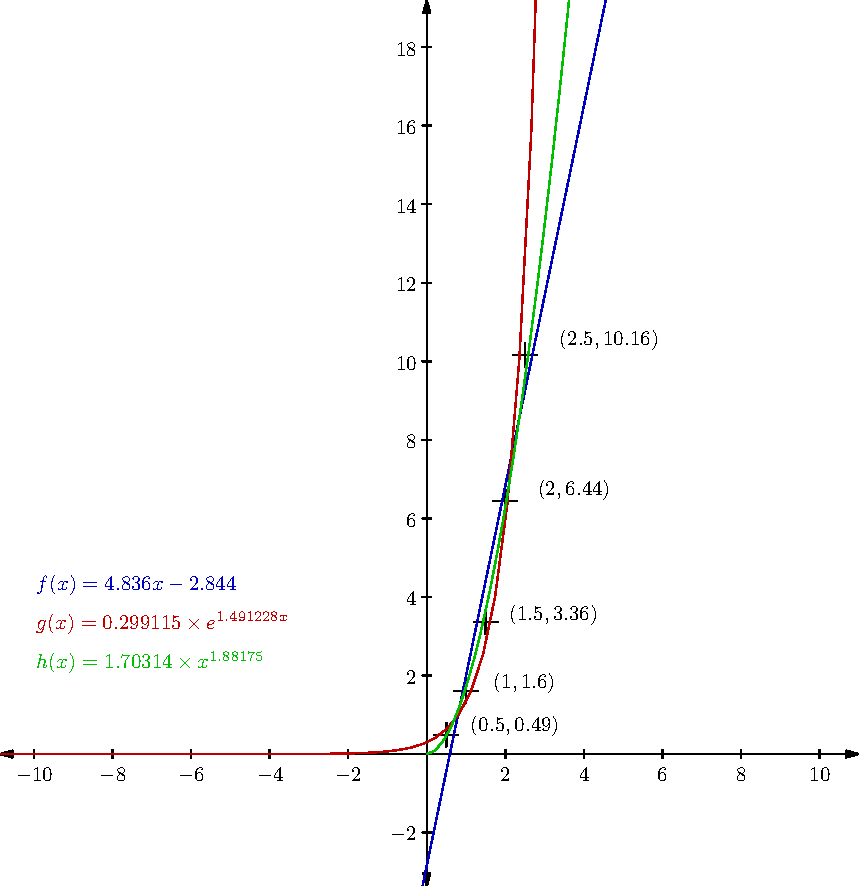
\includegraphics{graphiques/pdf_output/reglin.pdf}
	  \caption{Régression linéaire -- (Tableau \ref{approx_td3_ex6})}
	\end{figure}
      \newpage
      \subsection{Série d'Anscombe}
	\begin{table}[h]
	  \centering
	  \begin{tabular}{| c | c | c | c | c | c | c | c | c | c | c | c |}
	    \hline 
	    $x_{i}$ & $10$ & $8$ & $13$ & $9$ & $11$ & $14$ & $6$ & $4$ & $12$ & $7$ & $5$ \\ 
	    \hline 
	    $y^{(A)}_{i}$ & $8.04$ & $6.95$ & $7.58$ & $8.81$ & $8.33$ & $9.96$ & $7.24$ & $4.26$ & $10.84$ & $4.82$ & $5.68$ \\ 
	    \hline 
	  \end{tabular}
	  \caption{Série dûe à Anscombe}
	  \label{approx_tp2_ex1}
	\end{table}
	\begin{figure}[h]
	  \centering
	  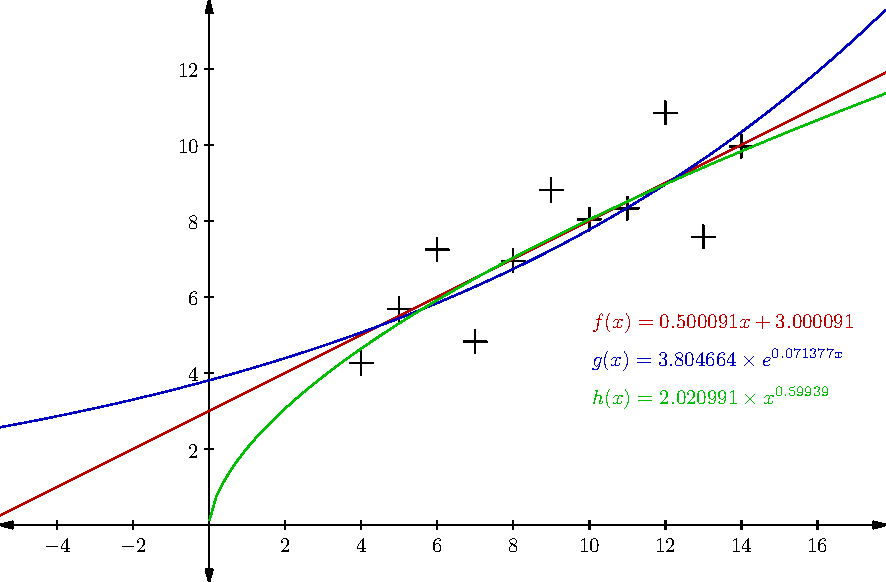
\includegraphics{graphiques/pdf_output/reglin_tp2_ex1.pdf}
	  \caption{Régression linéaire -- (Tableau \ref{approx_tp2_ex1})}
	\end{figure}
	\newpage
      \subsection{3 séries}
	\begin{table}[h]
	  \centering
	  \begin{tabular}{| c | c | c | c | c | c | c | c | c | c | c | c |}
	    \hline 
	    $x_{i}$ & $10$ & $8$ & $13$ & $9$ & $11$ & $14$ & $6$ & $4$ & $12$ & $7$ & $5$ \\ 
	    \hline 
	    $y^{(1)}_{i}$ & $9.14$ & $8.14$ & $8.74$ & $8.77$ & $9.26$ & $8.10$ & $6.13$ & $3.10$ & $9.13$ & $7.26$ & $4.74$ \\ %s1
	    \hline 
	    $y^{(2)}_{i}$ & $7.46$ & $6.77$ & $12.74$ & $7.11$ & $7.81$ & $8.84$ & $6.08$ & $5.39$ & $8.15$ & $6.42$ & $5.73$ \\ %s2
	    \hline 
	    $y^{(3)}_{i}$ & $6.58$ & $5.76$ & $7.71$ & $8.84$ & $8.47$ & $7.04$ & $5.25$ & $12.50$ & $5.56$ & $7.91$ & $6.89$ \\ %s3
	    \hline 
	    $y^{(A)}_{i}$ & $8.04$ & $6.95$ & $7.58$ & $8.81$ & $8.33$ & $9.96$ & $7.24$ & $4.26$ & $10.84$ & $4.82$ & $5.68$ \\ %anscombe
	    \hline 
	  \end{tabular}
	  \caption{3 séries $S^{(1)}$, $S^{(2)}$ et $S^{(3)}$ comparées à Anscombe}
	  \label{approx_tp2_ex2}
	\end{table}
	Série (1) :
	\newline
	Regression linéaire par une droite : $P(x) = 3.000909 + 0.500000 \cdot x$
	\newline
	Erreur moyenne : $0.967934$
	\newline
	\newline
	Série (2) :
	\newline
	Regression linéaire par une droite : $P(x) = 3.002455 + 0.499727 \cdot x$
	\newline
	Erreur moyenne : $0.715967$
	
	\begin{figure}[h]
	  \centering
	  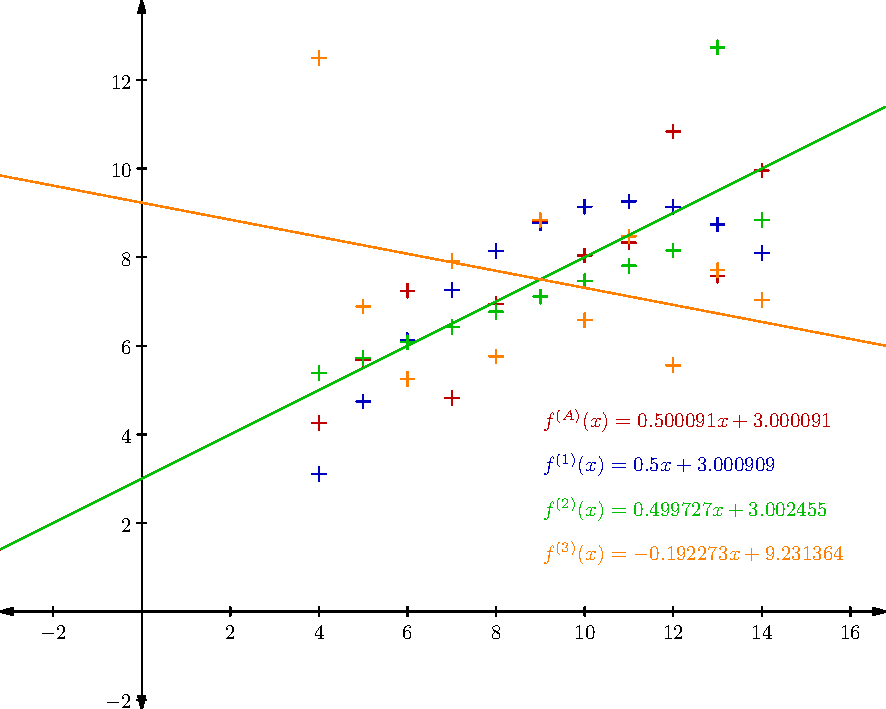
\includegraphics{graphiques/pdf_output/reglin_tp2_ex2_1.pdf}
	  \caption{Régression linéaire -- (Tableau \ref{approx_tp2_ex2})}
	\end{figure}
	\newpage
        Regression linéaire par une exponentielle :$P(x) = 3.417548 \cdot \exp(0.082249 \cdot x)$
        
        Erreur moyenne : $1.187786$

        Regression linéaire par une exponentielle :$P(x) = 4.100273 \cdot \exp(0.063981 \cdot x)$
        
        Erreur moyenne : $0.590601$

	\begin{figure}[h]
	  \centering
	  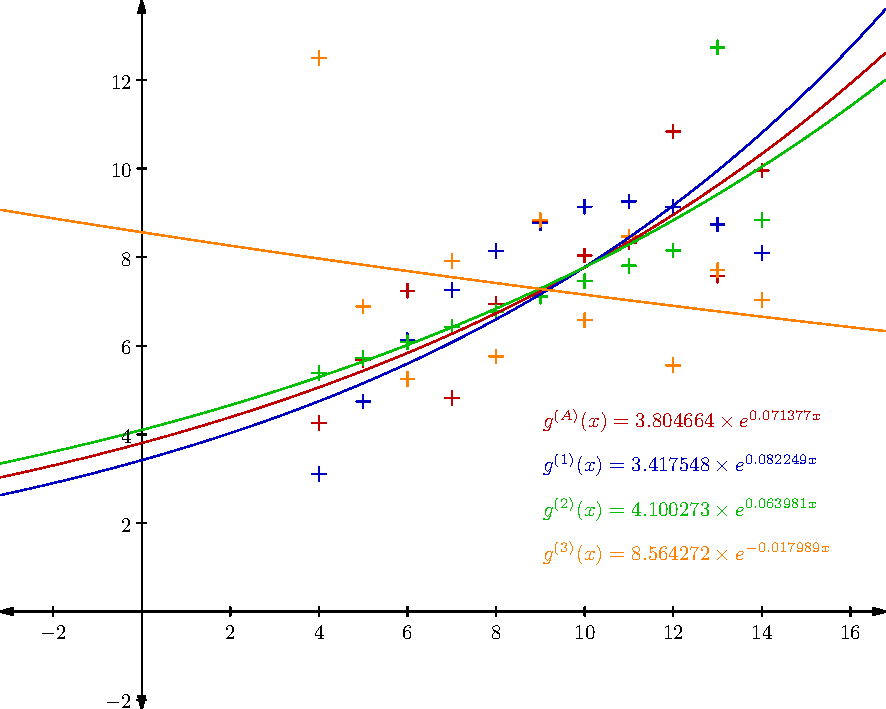
\includegraphics{graphiques/pdf_output/reglin_tp2_ex2_2.pdf}
	  \caption{Approximation par ajustement exponentiel -- (Tableau \ref{approx_tp2_ex2})}
	\end{figure}
	\newpage
        Regression linéaire par une puissance : $P(x) = 1.453451 \cdot x^{0.749910}$
        
        Erreur moyenne : $0.950634$

        Regression linéaire par une puissance :$P(x) = 2.478570 \cdot x^{0.507328}$
        
        Erreur moyenne : $0.682932$
	\begin{figure}[h]
	  \centering
	  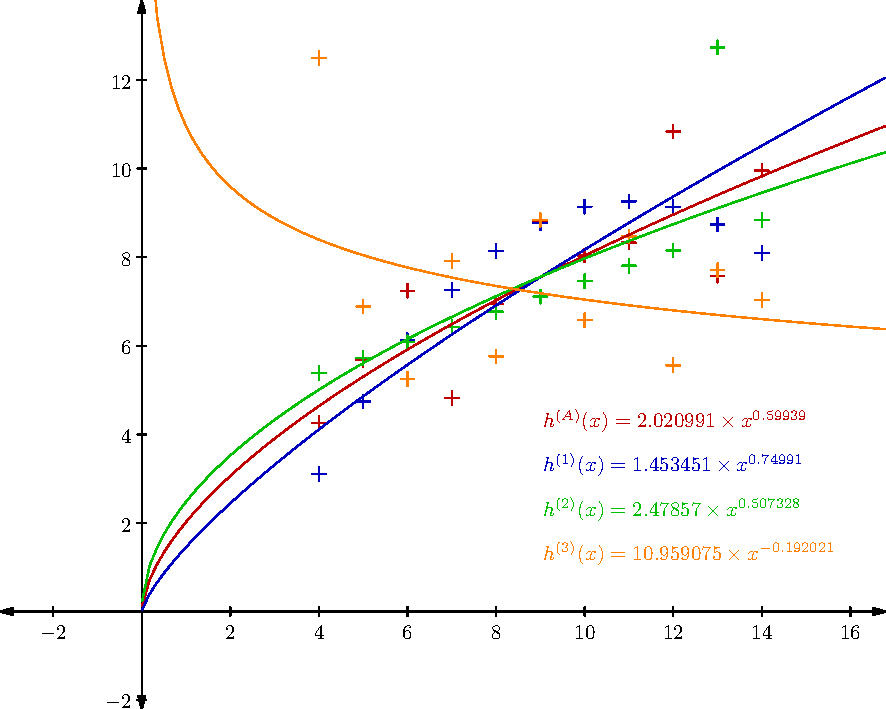
\includegraphics{graphiques/pdf_output/reglin_tp2_ex2_3.pdf}
	  \caption{Approximation par ajustement ``puissance" -- (Tableau \ref{approx_tp2_ex2})}
	\end{figure}
      \newpage
      \subsection{Dépenses mensuelles et revenus}
	\begin{table}[h]
	  \centering
	  \begin{tabular}{| c | c | c | c | c | c | c | c | c | c | c | c |}
	    \hline 
	    $x_{i}$ (R) & $752$ & $855$ & $871$ & $734$ & $610$ & $582$ & $921$ & $492$ & $569$ & $462$ & $907 $ \\ 
	    \hline 
	    $y_{i}$ (D) & $85$ & $83$ & $162$ & $79$ & $81$ & $83$ & $281$ & $81$ & $81$ & $80$ & $243 $ \\ 
	    \hline 
	  \end{tabular}
	  \caption{Série 1}
	  \label{approx_tp2_ex3_1}
	\end{table}
	\begin{table}[h]
	  \centering
	  \begin{tabular}{| c | c | c | c | c | c | c | c | c | c | c |}
	  \hline 
	  $x_{i}$ (R) & $643$ & $862$ & $524$ & $679$ & $902$ & $918$ & $828$ & $875$ & $809$ & $894$ \\ 
	  \hline 
	  $y_{i}$ (D) & $84$ & $84$ & $82$ & $80$ & $226$ & $260$ & $82$ & $186$ & $77$ & $223$ \\ 
	  \hline 
	  \end{tabular}
	  \caption{Série 2}
	  \label{approx_tp2_ex3_2}
	\end{table}
	Série 1 :
	\newline
	Regression linéaire par une droite :$ P(x) =  - 98.368005 + 0.312192 \cdot x$
	\newline
	Erreur moyenne : $38.488186$
	\newline
	\newline
	Regression linéaire par une exponentielle :$P(x) = 24.011644 \cdot \exp(0.002124 \cdot x)$
	\newline
	Erreur moyenne : $33.486916$
	\newline
	\newline
	Regression linéaire par une puissance :$P(x) = 0.015258 \cdot x^{1.356482}$
	\newline
	Erreur moyenne : $36.660388$
	\newline 
	\newline
	\newline
	Série 2 :
	\newline
	Regression linéaire par une droite :$P(x) =  - 164.266162 + 0.381480 \cdot x$
	\newline
	Erreur moyenne : $46.455702$
	\newline
	\newline
	Regression linéaire par une exponentielle :$P(x) = 14.780629 \cdot \exp(0.002657 \cdot x)$
	\newline
	Erreur moyenne : $45.099159$
	\newline
	\newline
	Regression linéaire par une puissance :$P(x) = 0.000785  \cdot x^{1.793989}$
	\newline
	Erreur moyenne : $47.682118$
  %       \begin{figure}[h]
  % 	\centering
  % 	\includegraphics[scale=0.7]{}
  % 	\caption{Approximation -- (Tableau \ref{Jeux d'essais approximation 3.3 Série 1})}
  %       \end{figure}
      \newpage
      
      \subsection{Série chronologique avec accroissement exponentiel}
      
      \newpage
      
      \subsection{Vérification de la loi de Pareto}

  \chapter{Conclusion}

\end{document}


      
%       \newpage      
%       \begin{table}[h]
% 	\centering
% 		\begin{tabular}{| c | c | c | c | c | c | c | c | c | c | c | c | c | c | c | c | c | c | c | c | c |}
% 	\hline 
% 	$x_{i}$ & $0$ & $2$ & $4$ & $6$ & $8$ & $10$ & $12$ & $14$ & $16$ & $18$ & $20$ & $22$ & $24$ & $26$ & $28$ & $30$ & $32$ & $34$ & $36$ & $38$ \\ 
% 	\hline 
% 	$y_{i}$ & $0.999870$ & $0.999970$ & $1$ & $0.999970$ & $0.999880$ & $0.999730$ & $0.999530$ & $0.999530$ & $0.998970$ & $0.998460$ & $0.998050$ & $0.999751$ & $0.997050$ & $0.996500$ & $0.996640$ & $0.995330$ & $0.994720$ & $0.994720$ & $0.993330$ & $0.993260$ \\ 
% 	\hline 
% 	\end{tabular}
% 	\caption{3.1 Densité de l'eau en fonction de la température}
% 	%\label{Jeux d'essais approximation 3.0}
% 		\end{table}
% 	
% 	Regression linéaire par une droite : $P(x) = 1.001302 - 0.000186 \cdot x$
% 	
% 	Erreur moyenne : $0.000665$
% 	
% 	Regression linéaire par une exponentielle : $P(x) = 1.001308 \cdot \exp(-0.000187 \cdot x) $
% 	
% 	Erreur moyenne : $0.000667$
% 	
% 	Regression linéaire par une puissance : Pas de résultat, lors du changement de variable, on calcule $\log_{2}(0)$ qui n'est pas défini.
	
	% 		\begin{figure}[h]
% 	\centering
% 	\includegraphics[scale=0.7]{graphiques/pdf_output/}
% 	\caption{Approximation -- (Tableau \ref{Jeux d'essais approximation 3.0})}
%       \end{figure}
%       \newpage
      
%       \begin{figure}[h]
% 	\centering
% 	\includegraphics[scale=0.7]{}
% 	\caption{Approximation-- (Tableau \ref{Jeux d'essais approximation 3.3 Série 2})}
%       \end{figure}


%       \newpage
%       \begin{table}[h]
% 	\centering
% 	\begin{tabular}{| c | c | c | c | c | c | c | c | c | c | c | c | c | c | c | c | c | c | c | c | c | c |}
% 	  \hline 
% 	  $x_{i}$ & $752$ & $855$ & $871$ & $734$ & $610$ & $582$ & $921$ & $492$ & $569$ & $462$ & $907$ & $643$ & $862$ & $524$ & $679$ & $902$ & $918$ & $828$ & $875$ & $809$ & $894$ \\ 
% 	  \hline 
% 	  $y_{i}$ & $85$ & $83$ & $162$ & $79$ & $81$ & $83$ & $281$ & $81$ & $81$ & $80$ & $243$ & $84$ & $84$ & $82$ & $80$ & $226$ & $260$ & $82$ & $186$ & $77$ & $223$ \\ 
% 	  \hline 
% 	\end{tabular}
% 	\caption{Série1-2 dépense}
% 	%\label{Jeux d'essais interpolation 3.3 Série 1 et 2}
%       \end{table}
% 	Regression linéaire par une droite :$P(x) =  - 112.658491 + 0.324356 \cdot x$
% 	
% 	Erreur moyenne : $43.378231$
% 	
% 	Reression linéaire par une exponentielle :$P(x) = 21.399929\cdot \exp(0.002238 \cdot x)$
% 	
% 	Erreur moyenne : $40.094599$
% 	
% 	Regression linéaire par une puissance :$P(x) = 0.007872 \cdot x^{1.453059}$
% 	
% 	Erreur moyenne : $42.696155$
%       
%       \begin{figure}[h]
% 	\centering
% 	\includegraphics[scale=0.7]{}
% 	\caption{Approximation -- (Tableau \ref{Jeux d'essais interpolation 3.3 Série 1 et 2})}
%       \end{figure}
